\documentclass[]{article}
\usepackage{lmodern}
\usepackage{amssymb,amsmath}
\usepackage{ifxetex,ifluatex}
\usepackage{fixltx2e} % provides \textsubscript
\ifnum 0\ifxetex 1\fi\ifluatex 1\fi=0 % if pdftex
  \usepackage[T1]{fontenc}
  \usepackage[utf8]{inputenc}
\else % if luatex or xelatex
  \ifxetex
    \usepackage{mathspec}
  \else
    \usepackage{fontspec}
  \fi
  \defaultfontfeatures{Ligatures=TeX,Scale=MatchLowercase}
\fi
% use upquote if available, for straight quotes in verbatim environments
\IfFileExists{upquote.sty}{\usepackage{upquote}}{}
% use microtype if available
\IfFileExists{microtype.sty}{%
\usepackage{microtype}
\UseMicrotypeSet[protrusion]{basicmath} % disable protrusion for tt fonts
}{}
\usepackage[margin=1in]{geometry}
\usepackage{hyperref}
\PassOptionsToPackage{usenames,dvipsnames}{color} % color is loaded by hyperref
\hypersetup{unicode=true,
            pdftitle={Exponential Distribution and Central Limit Theorem},
            pdfauthor={Thomas Fischer},
            colorlinks=true,
            linkcolor=blue,
            citecolor=Blue,
            urlcolor=Blue,
            breaklinks=true}
\urlstyle{same}  % don't use monospace font for urls
\usepackage{color}
\usepackage{fancyvrb}
\newcommand{\VerbBar}{|}
\newcommand{\VERB}{\Verb[commandchars=\\\{\}]}
\DefineVerbatimEnvironment{Highlighting}{Verbatim}{commandchars=\\\{\}}
% Add ',fontsize=\small' for more characters per line
\usepackage{framed}
\definecolor{shadecolor}{RGB}{248,248,248}
\newenvironment{Shaded}{\begin{snugshade}}{\end{snugshade}}
\newcommand{\KeywordTok}[1]{\textcolor[rgb]{0.13,0.29,0.53}{\textbf{#1}}}
\newcommand{\DataTypeTok}[1]{\textcolor[rgb]{0.13,0.29,0.53}{#1}}
\newcommand{\DecValTok}[1]{\textcolor[rgb]{0.00,0.00,0.81}{#1}}
\newcommand{\BaseNTok}[1]{\textcolor[rgb]{0.00,0.00,0.81}{#1}}
\newcommand{\FloatTok}[1]{\textcolor[rgb]{0.00,0.00,0.81}{#1}}
\newcommand{\ConstantTok}[1]{\textcolor[rgb]{0.00,0.00,0.00}{#1}}
\newcommand{\CharTok}[1]{\textcolor[rgb]{0.31,0.60,0.02}{#1}}
\newcommand{\SpecialCharTok}[1]{\textcolor[rgb]{0.00,0.00,0.00}{#1}}
\newcommand{\StringTok}[1]{\textcolor[rgb]{0.31,0.60,0.02}{#1}}
\newcommand{\VerbatimStringTok}[1]{\textcolor[rgb]{0.31,0.60,0.02}{#1}}
\newcommand{\SpecialStringTok}[1]{\textcolor[rgb]{0.31,0.60,0.02}{#1}}
\newcommand{\ImportTok}[1]{#1}
\newcommand{\CommentTok}[1]{\textcolor[rgb]{0.56,0.35,0.01}{\textit{#1}}}
\newcommand{\DocumentationTok}[1]{\textcolor[rgb]{0.56,0.35,0.01}{\textbf{\textit{#1}}}}
\newcommand{\AnnotationTok}[1]{\textcolor[rgb]{0.56,0.35,0.01}{\textbf{\textit{#1}}}}
\newcommand{\CommentVarTok}[1]{\textcolor[rgb]{0.56,0.35,0.01}{\textbf{\textit{#1}}}}
\newcommand{\OtherTok}[1]{\textcolor[rgb]{0.56,0.35,0.01}{#1}}
\newcommand{\FunctionTok}[1]{\textcolor[rgb]{0.00,0.00,0.00}{#1}}
\newcommand{\VariableTok}[1]{\textcolor[rgb]{0.00,0.00,0.00}{#1}}
\newcommand{\ControlFlowTok}[1]{\textcolor[rgb]{0.13,0.29,0.53}{\textbf{#1}}}
\newcommand{\OperatorTok}[1]{\textcolor[rgb]{0.81,0.36,0.00}{\textbf{#1}}}
\newcommand{\BuiltInTok}[1]{#1}
\newcommand{\ExtensionTok}[1]{#1}
\newcommand{\PreprocessorTok}[1]{\textcolor[rgb]{0.56,0.35,0.01}{\textit{#1}}}
\newcommand{\AttributeTok}[1]{\textcolor[rgb]{0.77,0.63,0.00}{#1}}
\newcommand{\RegionMarkerTok}[1]{#1}
\newcommand{\InformationTok}[1]{\textcolor[rgb]{0.56,0.35,0.01}{\textbf{\textit{#1}}}}
\newcommand{\WarningTok}[1]{\textcolor[rgb]{0.56,0.35,0.01}{\textbf{\textit{#1}}}}
\newcommand{\AlertTok}[1]{\textcolor[rgb]{0.94,0.16,0.16}{#1}}
\newcommand{\ErrorTok}[1]{\textcolor[rgb]{0.64,0.00,0.00}{\textbf{#1}}}
\newcommand{\NormalTok}[1]{#1}
\usepackage{longtable,booktabs}
\usepackage{graphicx,grffile}
\makeatletter
\def\maxwidth{\ifdim\Gin@nat@width>\linewidth\linewidth\else\Gin@nat@width\fi}
\def\maxheight{\ifdim\Gin@nat@height>\textheight\textheight\else\Gin@nat@height\fi}
\makeatother
% Scale images if necessary, so that they will not overflow the page
% margins by default, and it is still possible to overwrite the defaults
% using explicit options in \includegraphics[width, height, ...]{}
\setkeys{Gin}{width=\maxwidth,height=\maxheight,keepaspectratio}
\IfFileExists{parskip.sty}{%
\usepackage{parskip}
}{% else
\setlength{\parindent}{0pt}
\setlength{\parskip}{6pt plus 2pt minus 1pt}
}
\setlength{\emergencystretch}{3em}  % prevent overfull lines
\providecommand{\tightlist}{%
  \setlength{\itemsep}{0pt}\setlength{\parskip}{0pt}}
\setcounter{secnumdepth}{0}
% Redefines (sub)paragraphs to behave more like sections
\ifx\paragraph\undefined\else
\let\oldparagraph\paragraph
\renewcommand{\paragraph}[1]{\oldparagraph{#1}\mbox{}}
\fi
\ifx\subparagraph\undefined\else
\let\oldsubparagraph\subparagraph
\renewcommand{\subparagraph}[1]{\oldsubparagraph{#1}\mbox{}}
\fi

%%% Use protect on footnotes to avoid problems with footnotes in titles
\let\rmarkdownfootnote\footnote%
\def\footnote{\protect\rmarkdownfootnote}

%%% Change title format to be more compact
\usepackage{titling}

% Create subtitle command for use in maketitle
\newcommand{\subtitle}[1]{
  \posttitle{
    \begin{center}\large#1\end{center}
    }
}

\setlength{\droptitle}{-2em}
  \title{Exponential Distribution and Central Limit Theorem}
  \pretitle{\vspace{\droptitle}\centering\huge}
  \posttitle{\par}
  \author{Thomas Fischer}
  \preauthor{\centering\large\emph}
  \postauthor{\par}
  \predate{\centering\large\emph}
  \postdate{\par}
  \date{May 30, 2018}


\begin{document}
\maketitle
\begin{abstract}
\textbf{\emph{This document provides the assignment `Course Project Part
1' for Coursera's Statistical Inference Class in the Coursera Data
Science series. Replication files are available on the author's Github
account (\url{https://github.com/tomfischersz}).}}
\end{abstract}

\section{1. Synopsis}\label{synopsis}

The aim of this report is to investigate the sampling distribution for
\(\bar X_n\), derived as the mean from samples with size \(n\) from an
exponential distribution. The Central Limit Theorem (CLT) states, that
for large \(n\) we should except our sampling distribution to be
approximately normal with mean \(\mu_{\bar X} =\mu\) and standard
deviation \(\sigma_{\bar X} =\)\(\frac{\sigma}{\sqrt{n}}\) (also called
standard error of the mean).

\section{2. Simulation}\label{simulation}

The first step is to simulate 1000 random variables each calculated as
the mean of \(n = 40\) random exponential variables with population
parameter \(\lambda = 0.2\) (rate). To generate random exponential
variables we use the R function rexp(). The resulting 1000 sample means,
which themselves are random variables, are stored in a vector
(\protect\hyperlink{Appendix_1}{Code}).

\section{3. Sample Mean versus Theoretical
Mean}\label{sample-mean-versus-theoretical-mean}

The theoretical mean is the population mean of our exponential
distribution with \(\lambda = 0.2\) and is given as
\(\mu = \frac{1}{\lambda}\). According to the Law of Large Numbers we
also know that the sampling distribution for \(\bar X_n\) is centered at
\(\mu\), therefore \(\mu_{\bar X} = \frac{1}{\lambda}\). We can now
compare this theoretical mean with the actual mean of the simulation of
1000 means from samples of size 40
(\protect\hyperlink{Appendix_2}{Code}). The following table shows, that
the two calculated values are very close to each other:

\begin{longtable}[]{@{}lll@{}}
\toprule
Theoretical Mean & Sample Mean & Deviation from
Theoretical\tabularnewline
\midrule
\endhead
5 & 5.0034469 & 0.07 \%\tabularnewline
\bottomrule
\end{longtable}

\section{4. Sample Variance versus Theoretical
Variance}\label{sample-variance-versus-theoretical-variance}

We now have a closer look at the variability or spread of our sampling
distribution of means. The theoretical variance of the mean of samples
with size \(n\) from iid random exponential variables is given as
\(VAR(\bar X) = \frac{\sigma^2}{n}\), where \(\sigma^2\) is the variance
of the population we sampled from which is \(\frac{1}{\lambda^2}\). We
therefore can rewrite \(VAR(\bar X) = \frac{1}{\lambda^2 n}\). We
calculate the theoretical variance and the actual variance
(\protect\hyperlink{Appendix_4}{Code}) and show it as a table:

\begin{longtable}[]{@{}lll@{}}
\toprule
Theoretical Variance & Actual Variance & Deviation from
Theoretical\tabularnewline
\midrule
\endhead
0.625 & 0.6551711 & 4.83 \%\tabularnewline
\bottomrule
\end{longtable}

\section{5. Distribution}\label{distribution}

Finally we want to examine if the distribution of our simulation of 1000
averages of 40 random exponentials is approximately normal. In figure
\ref{fig:fig_hist_1} we plot the histogram of our simulation data
together with the theoretical normal distribution we would except
according to the CLT. In figure \ref{fig:fig_qqnorm} we plot a Q-Q
(Quantile-Quantile) Plot, where we compare the theoretical quantiles
with observed quantiles.

\begin{figure}[h]

{\centering 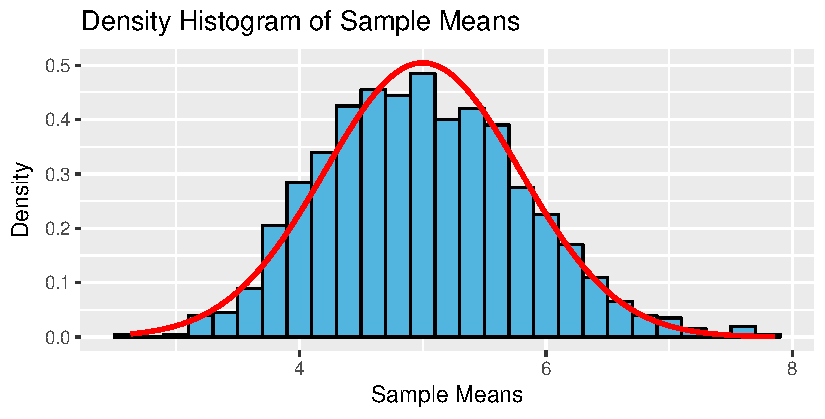
\includegraphics{exponential_distribution_files/figure-latex/plot_hist_1-1} 

}

\caption{\label{fig:fig_hist_1}Sampling distribution of the sample mean. The red line shows the standard normal pdf we would except according the CLT.}\label{fig:plot_hist_1}
\end{figure}

\begin{figure}[h]

{\centering 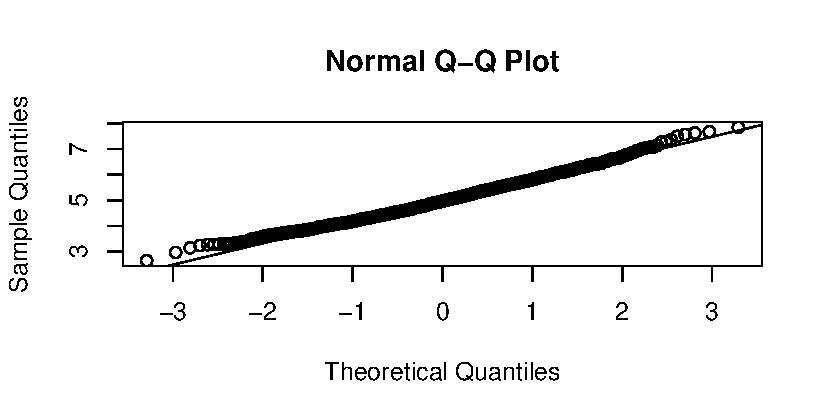
\includegraphics{exponential_distribution_files/figure-latex/unnamed-chunk-5-1} 

}

\caption{\label{fig:fig_qqnorm}Quantile-Quantile Plot of the observed sampling distribution of the sample mean versus a normal distribution with mean = 5 and standard deviation = 0.79.}\label{fig:unnamed-chunk-5}
\end{figure}

\section{6. Conclusion}\label{conclusion}

The histogram of our sample means in figure \ref{fig:fig_hist_1} shows a
density distribution that is quite normal and the Q-Q Plot in figure
\ref{fig:fig_qqnorm} shows a nearly linear plot. That let us conclude
that in fact our simulated distribution of 1000 averages of 40 random
exponential variables follows quite good a normal gaussian distribution
\({N}(5, \frac{5}{\sqrt{40}})\). That is what we expected from the
Central Limit Theorem.

\newpage

\section{Appendix: R Source Code}\label{appendix-r-source-code}

\hypertarget{Appendix_1}{\subsubsection{1. Code for creating our
simulation:}\label{Appendix_1}}

\begin{Shaded}
\begin{Highlighting}[]
\NormalTok{lambda <-}\StringTok{ }\FloatTok{0.2} \CommentTok{# rate parameter}
\NormalTok{n <-}\StringTok{ }\DecValTok{40} \CommentTok{# sample size}
\NormalTok{no_simulations <-}\StringTok{ }\DecValTok{1000} \CommentTok{# number of samples}
\KeywordTok{set.seed}\NormalTok{(}\DecValTok{1347}\NormalTok{)}
\NormalTok{sample_means <-}\StringTok{ }\KeywordTok{replicate}\NormalTok{(}\DataTypeTok{n =}\NormalTok{ no_simulations, }\KeywordTok{mean}\NormalTok{(}\KeywordTok{rexp}\NormalTok{(n, }\DataTypeTok{rate =}\NormalTok{ lambda)))}
\end{Highlighting}
\end{Shaded}

\hypertarget{Appendix_2}{\subsubsection{2. Calculating the theoretical
mean and the mean of the 1000 sample means:}\label{Appendix_2}}

\begin{Shaded}
\begin{Highlighting}[]
\NormalTok{theoretical_mu <-}\StringTok{ }\DecValTok{1}\OperatorTok{/}\NormalTok{lambda}
\NormalTok{mu_sample_means <-}\StringTok{ }\KeywordTok{mean}\NormalTok{(sample_means)}
\NormalTok{dev_mean <-}\StringTok{ }\KeywordTok{paste}\NormalTok{(}\KeywordTok{round}\NormalTok{((mu_sample_means }\OperatorTok{-}\StringTok{ }\NormalTok{theoretical_mu) }\OperatorTok{/}
\StringTok{                            }\NormalTok{theoretical_mu }\OperatorTok{*}\StringTok{ }\DecValTok{100}\NormalTok{, }\DecValTok{2}\NormalTok{),}\StringTok{'%'}\NormalTok{)}
\end{Highlighting}
\end{Shaded}

\hypertarget{Appendix_4}{\subsubsection{3. Calculating theoretical and
actual variance:}\label{Appendix_4}}

\begin{Shaded}
\begin{Highlighting}[]
\NormalTok{theoretical_var <-}\StringTok{ }\DecValTok{1}\OperatorTok{/}\NormalTok{(lambda}\OperatorTok{^}\DecValTok{2} \OperatorTok{*}\StringTok{ }\NormalTok{n)}
\NormalTok{var_sample_means <-}\StringTok{ }\KeywordTok{var}\NormalTok{(sample_means)}
\NormalTok{dev_variance <-}\StringTok{ }\KeywordTok{paste}\NormalTok{(}\KeywordTok{round}\NormalTok{((var_sample_means }\OperatorTok{-}\StringTok{ }\NormalTok{theoretical_var) }\OperatorTok{/}
\StringTok{                                }\NormalTok{theoretical_var }\OperatorTok{*}\StringTok{ }\DecValTok{100}\NormalTok{, }\DecValTok{2}\NormalTok{),}\StringTok{'%'}\NormalTok{)}
\end{Highlighting}
\end{Shaded}

\subsubsection{4. Histogram 1:}\label{Appendix_5}

\begin{Shaded}
\begin{Highlighting}[]
\NormalTok{hist_}\DecValTok{1}\NormalTok{ <-}\StringTok{ }\KeywordTok{ggplot}\NormalTok{(}\DataTypeTok{data =} \KeywordTok{data.frame}\NormalTok{(sample_means), }\KeywordTok{aes}\NormalTok{(}\DataTypeTok{x=}\NormalTok{sample_means))}
\NormalTok{hist_}\DecValTok{1}\NormalTok{ <-}\StringTok{ }\NormalTok{hist_}\DecValTok{1} \OperatorTok{+}\StringTok{ }\KeywordTok{geom_histogram}\NormalTok{(}\DataTypeTok{color =} \StringTok{'black'}\NormalTok{, }\DataTypeTok{binwidth =} \FloatTok{0.2}\NormalTok{,}
                                  \DataTypeTok{fill =} \StringTok{'#51B5E0'}\NormalTok{, }\KeywordTok{aes}\NormalTok{(}\DataTypeTok{y=}\NormalTok{..density..))}
\NormalTok{hist_}\DecValTok{1}\NormalTok{ <-}\StringTok{ }\NormalTok{hist_}\DecValTok{1} \OperatorTok{+}\StringTok{ }\KeywordTok{labs}\NormalTok{(}\DataTypeTok{x =} \StringTok{"Sample Means"}\NormalTok{,}
                        \DataTypeTok{y =} \StringTok{"Density"}\NormalTok{,}
                        \DataTypeTok{title =} \StringTok{"Density Histogram of Sample Means"}\NormalTok{)}
\NormalTok{hist_}\DecValTok{1}\NormalTok{ <-}\StringTok{ }\NormalTok{hist_}\DecValTok{1} \OperatorTok{+}\StringTok{ }\KeywordTok{stat_function}\NormalTok{(}\DataTypeTok{fun =}\NormalTok{ dnorm,}
                                 \DataTypeTok{args =} \KeywordTok{list}\NormalTok{(}\DataTypeTok{mean =}\NormalTok{ theoretical_mu,}
                                             \DataTypeTok{sd =} \KeywordTok{sqrt}\NormalTok{(theoretical_var)),}
                                 \DataTypeTok{colour =} \StringTok{"red"}\NormalTok{, }\DataTypeTok{size=}\DecValTok{1}\NormalTok{)}
\end{Highlighting}
\end{Shaded}

\subsubsection{5. Q-Q Plot}\label{q-q-plot}

\begin{Shaded}
\begin{Highlighting}[]
\KeywordTok{qqnorm}\NormalTok{(sample_means, }\DataTypeTok{main =} \StringTok{"Normal Q-Q Plot"}\NormalTok{)}
\KeywordTok{qqline}\NormalTok{(sample_means)}
\end{Highlighting}
\end{Shaded}


\end{document}
